
\subsection{Соединения элементов 1 группы, способы получения, химическое поведение, электронное строение и структура в различных фазах.}

\subsubsection*{$H_2$}

\textbf{Получение}

1) В промышленности

$$CH_4 + H_2O \xrightarrow[Ni]{1250K} CO + H_2$$
$$C_{tv} + H_2O_{gas} \xrightarrow{1300K} CO + H_2$$
$$CO + H_2O_{gas} \xrightarrow[FeSO_4]{675K} CO_2 + H_2$$

2) В лаборатории

$$CaH_2 + H_2O \rightarrow Ca(OH)_2 + H_2$$
$$Zn + H_2SO_{4(razb)} \rightarrow ZnSO_4 + H_2$$
$$Al + NaOH + H_2O \rightarrow Na[Al(OH)_4(H_2O)_2] + H_2$$
$$H_2O \rightarrow H_2 + O_2$$
$$NaCl + H_2O \rightarrow NaOH + H_2 + Cl_2$$

\textbf{Химические свойства}

Реакционная способность низка

1) С галогенами

$$H_2 + X_2 \rightarrow HX(X = F, Cl, Br, I)$$

2) С $O_2$ и $S$

$$H_2 + O_2 \xrightarrow{550^{\circ}} H_2O$$
$$H_2 + S \xrightarrow{150^{\circ}} H_2S$$

3) С $N_2$

Процесс Боша-Хабера

$$N_2 + H_2 \leftrightarrows NH_3$$\\
p = 200 атм, $T = 450^{\circ}C$, кат.смесь $Fe_3O_4 + Al_2O_3 + K_2O + SiO_2$

4) Восстановление MeO

$$Fe_3O_4  + H_2 \rightarrow Fe + H_2O$$

5) С Me - до гидридов

6) С соединениями, содержащими двойную связь (катализатор - поверхность металла)

\textbf{Строение}

Солнце и звёзды - атомарное состояние\\
Межзвёздное пространство - частично ионизированные двухатомные молекулы\\
Верхние слои атмосферы Земли - простое вещество (следствие количества)\\
Атмосфера Юпитера/Сатурна - ионы $H_3^+$; металлический водород\\
Большая часть на Земле - связан с водой

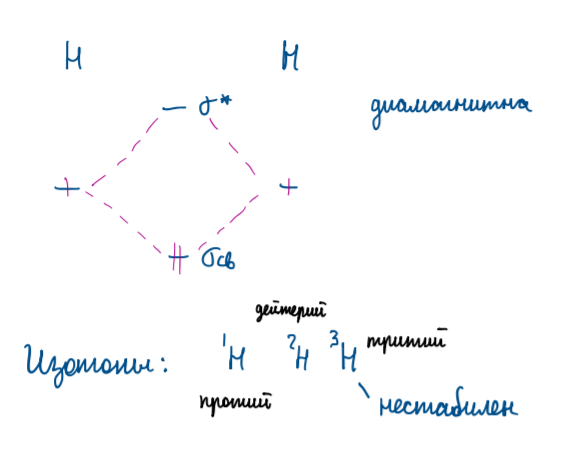
\includegraphics{images/11v13.png}
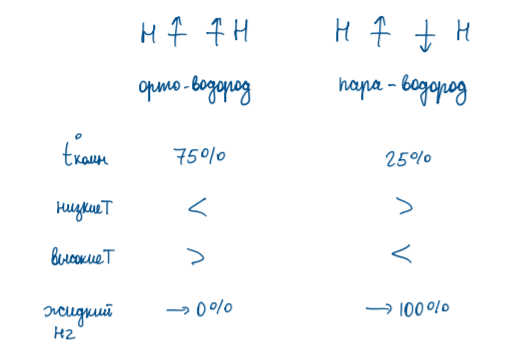
\includegraphics[scale=0.95]{images/11v14.png}

\subsubsection*{Гидриды}

\textbf{Ионные(солеобразные) - наиблее электрополоижетльные Ме (Щ и ЩЗ)}

\textbf{Получение}

$$Me + H_2 \rightarrow MeH(MeH_2)$$
$$Li + H_2 \xrightarrow{500-700^{\circ}} LiH$$

\textbf{Химические свойства}

1) Воспламеняются при растирании на воздухе

$$CaH_2 + O_2 \rightarrow CaO + H_2O$$

2) Легко разлагаются водой

$$NaH + H_2O \rightarrow NaOH + H_2$$

3) С кислотами Льюиса

$$LiH + AlCl_3 \xrightarrow{Et_2O} Li[AlH_4] + LiCl$$
$$NaH + BCl_3 \xrightarrow{THF} Na[BH_4] + NaCl$$

4) Термическое разложение

$$NaH \rightarrow Na + H_2$$

5) С $N_2$

$$CaH_2 + N_2 \rightarrow Ca_3N_2 + H_2$$

\textbf{Строение}

Кристаллическая решетка типа NaCl\\
При н.у. - устойчивы, при нагревании - разложение без плавления(Кроме $LiH, CaH_2$)

\textbf{Ковалентные}

Ковалентные - состоят из молекул или имеют полимерное строение\\
Молекулярное строение- гидриды неметаллов (13-17 группа)\\
Газы или летучие жидкости (зависит от элемента)\\
Разлагаются при нагревании, высокая реакционная способность, сильные восстановители

Полимерное строение - Be, Mg, Al, Zn,..\\
Гидрид-ионы мостиковые, образуются зс2е - связи


\includegraphics{images/12v1.png}

Получить прямым синтезом, как правило, нельзя\\
$$ZnI_2 + Li[AlH_4] \xrightarrow{Et_2O} ZnH_2 + LiI + AlI_3$$
$$CuSO_4 + H_3PO_2 + H_2O \rightarrow CuH + H_3PO_4 + H_2SO_4$$

Устойчивы к действию влаги и разбавленных кислот


\textbf{Металлические}

Металлические гидриды часто по физ.свойствам напоминают металлы.\\
Нестехиометрические составы\\
Очень прочная хим.связь, это примеры гипервалентных соединений\\
Способны поглощать большое количество H

$$Yb + H_2 \rightarrow YbH_2$$
$$LaNi_5 \leftrightarrows LaNi_5H_6$$

\subsubsection*{$H_2O$}

\textbf{Способы получения}

1) Продукт в огромном количестве реакций

2) Физические методы (дистилляция)

3) $H_2 + O_2 \rightarrow H_2O$

\textbf{Химические свойства}

1) Автопротолиз

$$2H_2O \leftrightarrows H_3O^+ + OH^-$$

2) Окислитель

$$H_2O + Al \rightarrow Al(OH)_3 + H_2$$

4) Восстановитель

$$H_2O + CoF_3 \rightarrow CoF_2 + O_2 + HF$$

\textbf{Электронное и геометрическое строение}

а) Лёд - гексагональная структура, каждая молекула воды связано с 3 соседними через н-связи; образуется прочный каркас; каждая молекула $H_2O$ участвует в образовании двух н-связей, используя обе НЭП

б) 0<t<4 плавление приводит к частичному разрушение каркаса, молекулы  $H_2O$ попадают в пустоты, и плотность растет (при $4^{\circ}C$ максимум)

в) 4<t<100 межмолекулярное взамодействие за счет одной НЭП на $B_1^0$; каждая молекула связана с тремя соседними

г) Пар - в основном, неассоциированные молекулы $H_2O$ и лишь немного димеров $(H_2O)_2$

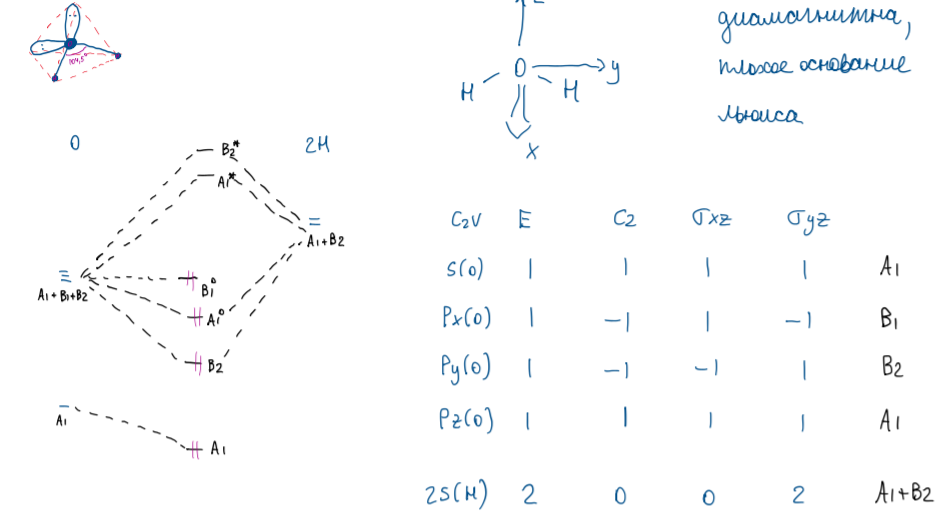
\includegraphics{images/12v2.png}

\subsubsection*{$H_2O_2$}

\textbf{Методы получения}

$$BaO_2 + H_2SO_4 \rightarrow BaSO_4\downarrow + H_2O_2$$
$$ (CH_3)_2CHOH + O_2 \rightarrow (CH_3)_2CO + H_2O_2$$

Окисление гидроантрахинонаксилородом воздуха в органическом растворителе

\textbf{Химические свойства}

1) Разложение
$$H_2O_2 \rightarrow H_2O + O_2$$

2) Слабая кислота

$$H_2O_2 + H_2O \rightarrow H_3O^+ + HO_2^-$$
$$H_2O_2 + NaOH \rightarrow Na_2O_2 + H_2O$$

3) $Red/ox$ свойства

- сильный окислитель в кислой среде

$$NaI + H_2O_2 + H_2SO_4 \rightarrow I_2 + Na_2SO_4 + H_2O$$

- Восстановитель в кислой среде

$$KMnO_4 + H_2O_2 + H_2SO_4 \rightarrow MnSO_4 + K_2SO_4 + H_2O + O_2$$

- Окислитель в щелочной среде

$$Cr(OH)_3 + H_2O_2 + KOH \rightarrow K2CrO_4 + H_2O$$

- Восстановитель в щелочной среде

$$KOH + Cl_2 + H_2O_2 \rightarrow KCl + O_2 + H_2O$$

- Гетерогенный окислитель

$$PbS_{tv.} + H_2O_2 \rightarrow PbSO_4{tv.} + H_2O$$

\textbf{Электронное и геометрическое строение}

Строение обусловлено взаимным отталкиванием между неподеленными парами $e^-$ O и $e^-$ связи $O-H$

Молекула сильно полярна

НЭП 0 $\Rightarrow$ Д/А связи

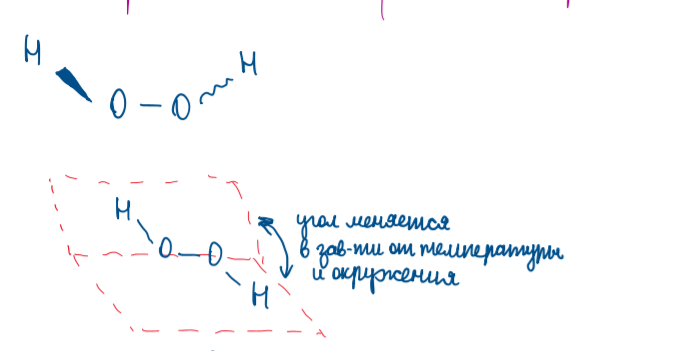
\includegraphics[scale=0.95]{images/6v3.png}

\subsubsection*{Металлы}

\textbf{Получение}

\textbf{Na}

Процесс Даунса:

$$NaCl + CaCl_2 \xrightarrow{580^{\circ}, razryad}$$

\textbf{Li}

$$Li_2O + Si + CaO \rightarrow Ca_2SiO_4  + Li$$
$$LiCl \rightarrow Li + Cl_2$$

\textbf{K}

$$KOH + Na \xrightarrow{N_2, 250^{\circ}} NaOH + K$$
$$KF + CaC_2 \rightarrow CaF_2 + C + K$$

\textbf{Cs, Rb = x}

$$XCl + Ca \rightarrow CaCl_2 + X$$

\textbf{Cs}

$$Cs_2CO_3 + Zr \rightarrow ZrO_2 + CO_2 + Cs$$

\textbf{Все кроме Li}

$$NaN_3 \rightarrow Me + N_2$$

\textbf{Химические свойства}

1) С $H_2O$ - бурно для всех Ме

$$Me + H_2O \rightarrow MeOH + H_2$$

2) Горение - всегда до смеси оксидов; основные компоненты:

$Li-Li_2O, Na - Na_2O_2, X - XO_2 (X = K, Cs, Rb)$

3)Образование озонидов

$$KOH + O_3 \xrightarrow{\leq20^{\circ}} KOH\cdot H_2O + O_2 + KO_3$$
4) С Hal - бурно

5) С $H_2$ - образование солеобразных гидридов

6) С кислотами

7) Растворение в $NH_{3(lig)}$

$$NaH + NH_3 \rightarrow H_2 + NaNH_2$$

$$Na_{solv}^+; e_{solv}^-$$

Для стабилизации ( испарения $NH_3$ и сохранения электрида) используют краун-эфиры

Ме не может иметь с.о. -1

\textbf{Особые свойства Li}

1) С $N_2$

$$Li + N_2 \rightarrow Li_3N$$

2) С $С$

$$Li + C \rightarrow Li_2C_3 / Li_4C_3$$
$$LiOH \xrightarrow{900^{\circ}} Li_2O + H_2O$$
$$Li_2CO_3 \xrightarrow{800^{\circ}} Li_2O + CO_2$$

3) Не образует квасцов, образует литиорганику

\textbf{Особые свойства Rb и Cs }

1) Образование субоксидов

$$Rb_2CO_3 + Rb \rightarrow Rb_9O_2 + CO$$

($Rb_6O; Cs_{11}O_3, Cs_4O; Cs_7O$)

\textbf{Строение}

Твердая фаза - объемно-центрированная кристаллическая решетка с металлическим типом хим.связи

Раствор - сольватированные ионы $[M(H_2O)_n]^+$

Прочность удерживания зависит от поляризующей способности $Me^+$

Например n(Li)=4, n(Cs)=12

Газ - атомы или двухатомные молекулы

\subsubsection*{Оксиды, пероксиды, надпероксиды, озониды}

\textbf{Получение}

1) $Me+ O_2$

Горение - всегда до смеси оксидов; основные компоненты:\\
$Li - Li_2O; Na - Na_2O_2; X-XO_2(X= K, Cs, Rb)$

2) Разложение пероксидов в вакууме или инертной атмосфере

3) $Me/MeN_3 + MeNO_2/MeNO_3 (t^{\circ})$

$$NaN_3 + NaNO_3 \rightarrow Na_2O + N_2$$
$$NaNO_2 \rightarrow Na_2O + N_2$$

$$NaOH + Na \rightarrow Na_2O + H_2$$
$$LiOH + H_2O_2 + H_2O \rightarrow LiOOH\cdot 3H_2O$$
$$LiOOH\cdot 3H_2O \xrightarrow{300^{\circ}} Li_2O_2 + H_2O + O_2$$

4) $XO_2 + O_3 \xrightarrow{\leq 20} X_2O (X= K, Cs, Rb)$

5) Получение озонидов

$$KOH + O_3 \xrightarrow{\leq 20^{\circ}} KOH\cdot H_2O + KO_3$$
$$KO_2 + O_3 \rightarrow KO_3 + O_2$$

\textbf{Химические свойства}

1) C $H_2O$

$$M_2O + H_2O \rightarrow MOH$$
$$M_2O_2 + H_2O \rightarrow MOH + H_2O_2$$
$$MO_2 + H_2O \rightarrow MOH + H_2O_2 + O_2$$
$$MO_3 + H_2O \rightarrow MOH + O_2$$

2) Разложение при нагревании перксидов, надперксидов и озонидов

$$M_2O_2 \rightarrow M_2O + O_2$$

3) Пероксиды и надпероксиды с $CO_2$

$$KO_2  + CO_2 \rightarrow K_2CO_3 + O_2$$

4) Пероксиды, надпероксиды и озониды - сильные окислители

$$Na_2O_2 + PbS + H_2SO_4 \rightarrow PbSO_4 + Na_2SO_4 + H_2O$$
$$Na_2O_2 + CO \rightarrow Na_2CO_3$$

\textbf{Строение}

1) Ионная кристаллическая решетка

2) $Me_2O_2 \ [O_2]^{2-}$ - диамагнитный

3) $MeO_2 [O_2]^- $ - парамагнитый

\subsubsection*{Гидроксиды}

\textbf{Получение}

$$NaCl + H_2O \rightarrow NaOH + H_2 + Cl_2$$
$$X_2SO_4 + Ba(OH)_2 \rightarrow BaSO_4 \downarrow + XOH (X=Rb,Cs)$$

\textbf{Химические свойства}

1) Растворимы в воде ( не  LiOH)

2) Плавятся без разложения
(но: $LiOH \xrightarrow[H_2]{800^{\circ}} + Li_2O + H_2O$)

3) С кислотами и кислотными оксидами

4) С Zn, Be, Al (до комплекса $H_2$)

5) С $Cl_2, S, P$ (диспропорционирование)

\textbf{Строение}

Все едкие щелочи образуют устойчивые гидраты, некоторые из них выделены в твердой фазе

Например, $LiOH\cdot H_2O$ построен из двойных цепочек

\subsubsection*{Соли}

Большинство солей элементов 1 группы хорошо растворимы в воде,\\
кроме солей $Li (F^-, CO_3^{2-}, SiO_3^{2-}, PO_4^{3-})$, солей $K^+, Rb^+, Cs^+$ с крупными анионами ($ClO_4^-, [PtCl_6]^{2-}, [PMo_{12}O_{40}]^{3-}, [SiW_{12}O_{40}]^{4-}$)

Нерастворимы соли $Na^+$ : $Na[Sb(OH)_6], NaM(UO_2)_3(CH_3COO)_9\cdot 6H_2O, (M = Mg, Zn)$

Важные значение имеет пищевая сода $NaHCO_3$

Производство по методу Сольве:
$$NaCl + H_2O + NH_3 + CO_2 \rightarrow NaHCO_3 + NH_4Cl$$
$$NaHCO_3 \xrightarrow{100^{\circ}} Na_2CO_3 + H_2O + CO_2$$

Кристаллы - комплексы щелочных металлов с N-, O-донорными полициклическими лигандами (криптандами), по сравнению с краун-эфирами > эффективно окружают $Me^+$ и более селективны

Ионы Ме удалось стабилизировать в алкалидах - соединений с криптандами (ионная структура)

При высокой концентрации криптанда образуется электриды - в их структуре в пустотах катионной решетки находятся сольватированные электроны
